\documentclass[11pt]{article}

\usepackage[margin=1.05in,top=1.15in,bottom=1.15in]{geometry}
\usepackage{booktabs,graphicx,xcolor,amsmath,amssymb}
\usepackage[most]{tcolorbox}
\usepackage{microtype,caption,longtable,array,enumitem,titlesec,fancyhdr,siunitx}
\usepackage{float}
\usepackage[hidelinks]{hyperref}

\definecolor{ink}{HTML}{1A1A1A}
\definecolor{accent}{HTML}{1F6F3F}
\definecolor{alert}{HTML}{C0392B}
\definecolor{muted}{HTML}{6B6B6B}
\definecolor{panel}{HTML}{F4F6F5}

\newtcolorbox{takeaway}[1]{colback=accent!6,colframe=accent!65,boxrule=0.7pt,
  left=7pt,right=7pt,top=6pt,bottom=6pt,arc=1.5pt,
  fonttitle=\bfseries\sffamily\small,title={#1}}
\newtcolorbox{caution}[1]{colback=alert!5,colframe=alert!60,boxrule=0.7pt,
  left=7pt,right=7pt,top=6pt,bottom=6pt,arc=1.5pt,
  fonttitle=\bfseries\sffamily\small,title={#1}}
\newtcolorbox{plainbox}{colback=panel,colframe=muted!45,boxrule=0.5pt,
  left=7pt,right=7pt,top=6pt,bottom=6pt,arc=1.5pt}

\titleformat{\section}{\Large\bfseries\sffamily\color{ink}}{\thesection}{0.7em}{}
\titleformat{\subsection}{\large\bfseries\sffamily\color{ink}}{\thesubsection}{0.6em}{}
\titlespacing*{\section}{0pt}{1.6em}{0.7em}

\pagestyle{fancy}\fancyhf{}
\lhead{\sffamily\scriptsize\color{muted}ARD36 — Multi-Agent Round Dynamics}
\rhead{\sffamily\scriptsize\color{muted}\thepage}
\renewcommand{\headrulewidth}{0.3pt}

\captionsetup{font=small,labelfont={bf,sf},width=0.95\textwidth}
\setlist[itemize]{leftmargin=1.2em,itemsep=2pt,topsep=3pt}
\sisetup{detect-weight=true}

\newcommand{\ci}[2]{\,[\,#1,\ #2\,]}
\newcommand{\rej}{\textcolor{alert}{\textbf{rejects}}}

\begin{document}

\begin{center}
{\LARGE\bfseries\sffamily What Communication Does to a Team of Agents}\\[4pt]
{\large\sffamily A characterization of multi-agent round dynamics, with emphasis on correct minorities}\\[10pt]
{\small\sffamily ARD36 study \textbullet\ 5 agents \textbullet\ 7 protocols \textbullet\ 4 rounds \textbullet\ Qwen3-8B/32B \textbullet\ MATH-500 + MMLU-Pro}\\[3pt]
{\footnotesize\color{muted}\sffamily Full report over the repaired tables (\texttt{tables\_v2}). Generated \today.}
\end{center}

\vspace{4pt}
\hrule
\vspace{10pt}

\begin{takeaway}{The result, in one paragraph}
A multi-agent team that lets its members read each other does \emph{not} find more right answers
than a team whose members only revise privately. It finds \emph{fewer}. Peer visibility costs
\textbf{4.6 percentage points} of team truth-coverage on a shared-root, item-paired design
(\(p=0.008\), Holm \(0.024\), \rej{} as a pre-registered primary). The mechanism is
\textbf{consolidation, not discovery}: communication concentrates agreement inside whichever
answer the team already holds --- the \emph{mean} number of correct agents rises while the
probability that \emph{anyone} is correct falls. The same signature appears independently in the
residual stream, where peer exchange contracts the team's representational spread, and the
contraction deepens monotonically with network depth.
\end{takeaway}

\vspace{2pt}

\begin{caution}{Read this before any number below}
This study was originally written up as \textbf{``all three pre-registered contrasts are null.''}
That was wrong. A cell-keying defect caused a 16-draw sampling bank to overwrite the round-0
baseline of the \textsc{private} arm, and the defect had a direction. After repair, one primary
inverts its sign and rejects. \textbf{Every number in this report comes from the repaired tables};
the frozen originals are quoted only to show what moved.
\end{caution}

\section{What this document is}

Between generation and analysis, this study accumulated a measurement problem large enough to
invert one of its own registered results. This report is the output of repairing that problem and
then re-characterizing the data from scratch.

\begin{plainbox}
\small
\textbf{Provenance.} Every figure and number derives from \texttt{tables\_v2/}, rebuilt from the
raw cell outputs after ten repairs (\S\ref{sec:repair}). The frozen \texttt{tables/} are
byte-identical to their state before this work began --- verified by SHA-256 on all 19 artifacts.
The regression suite is \textbf{1{,}519 passed / 1 skipped / 17 subtests}, up from a 1{,}336-test
baseline, with zero regressions.
\end{plainbox}

\paragraph{The evidence base.} 67{,}104 agent decisions across 4{,}888 episodes; 51{,}360 graded
answers; 240 held-out test items per arm; seven communication protocols sharing a
byte-identical round-0 root bank. Analysis enumerated \textbf{1{,}441 candidate trends}, of which
\textbf{692 were estimable}; 56 were computed and 39 were put through adversarial verification.

\paragraph{How claims were vetted.} Each computed claim was handed to an independent verifier
instructed to \emph{refute} it, attacking composition first. The yield was
\textbf{35 weakened, 4 refuted, 0 confirmed as originally stated}. Wherever a verifier disagreed
with an analyst, the verifier's wording is what appears here.

\section{The repair, and why it mattered}
\label{sec:repair}

\subsection{A defect that inverted a registered result}

\texttt{analysis.coverage\_change\_arm} accumulated per-episode coverage into a dictionary keyed on
\texttt{episode\_id} alone, and overwrote on collision. A \textsc{roots} cell --- the 16-draw
independent sampling bank --- defaults its protocol to \textsc{private} and shares an
\texttt{episode\_id} with the real \textsc{private} episode of the same item. The bank's round-0
coverage therefore replaced the five-agent team's round-0 coverage \emph{in the \textsc{private}
arm only}, inflating its baseline until \textsc{private} appeared to \emph{lose} coverage.

\begin{table}[H]\centering\small
\caption{The three pre-registered primary contrasts, before and after repair.}
\begin{tabular}{lcc}
\toprule
\textbf{Contrast} & \textbf{v1 (frozen)} & \textbf{v2 (repaired)} \\
\midrule
\textsc{gate}\,--\,\textsc{peer} (r3 accuracy) & $-0.0083$, $p{=}0.465$ & $-0.0089$, $p{=}0.396$ \\
\textsc{gate}\,--\,\textsc{random\_protect} & $-0.0258$, $p{=}0.056$ & $-0.0226$, $p{=}0.035$, Holm $0.071$ \\
\textbf{\textsc{peer}\,--\,\textsc{private} (coverage)} &
  $+0.0125$, $p{=}0.535$ & \textcolor{alert}{$\mathbf{-0.0458}$, $\mathbf{p{=}0.008}$, Holm $\mathbf{0.024}$, \rej} \\
\bottomrule
\end{tabular}
\end{table}

\begin{figure}[H]\centering
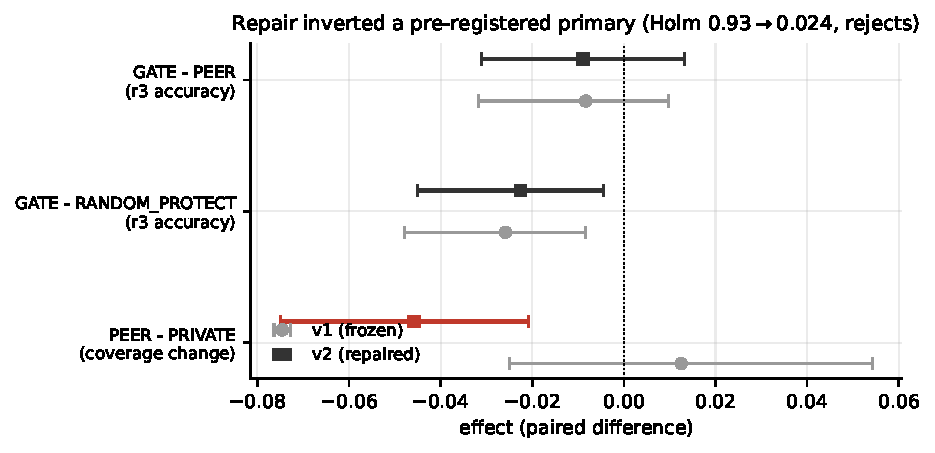
\includegraphics[width=0.80\textwidth]{figs/f3_signflip.pdf}
\caption{The repair moved one contrast across zero. The isolation is clean: \textsc{peer}'s
change is \emph{byte-identical} in v1 and v2 ($-0.02083$), because no \textsc{roots} cell aliases a
\textsc{peer} episode. Only \textsc{private} moved, from $-0.0333$ to $+0.0250$.}
\end{figure}

\begin{takeaway}{Three independent routes to the same number}
The repaired estimator gives $-0.04583$. A direct trajectory computation gives
$(77.92-80.00)-(82.50-80.00) = -4.58$\,pp. A root-paired exact McNemar on identical round-0 roots
gives \textbf{12 vs 1 discordant, $p = 0.0034$}. Three different code paths, one answer.
\end{takeaway}

\subsection{The other nine repairs}

\begin{table}[H]\centering\small
\caption{Repairs applied, each with the check that would have caught it failing.}
\begin{tabular}{p{0.30\textwidth}p{0.60\textwidth}}
\toprule
\textbf{Repair} & \textbf{Verification} \\
\midrule
Cell-kind keying (M2) & \texttt{(cell\_id, episode\_id, round)} unique on 12{,}832/12{,}832 \\
Tri-state correctness (M1) & 5{,}047 ungradeable no longer scored wrong; $C_{t+1}-C_t = WC-CW$ holds 6{,}771, \textbf{violated 0} \\
GPU-second attribution (B-1) & \textbf{268.75} request-hours $\rightarrow$ \textbf{25.41} attributed GPU-hours recovered \\
Fork re-metering & 1{,}440/1{,}440 recovered; FLOPs byte-identical; 0 mismatches on 263 control rows \\
Transition change rule & \textbf{40.0\%} of \texttt{changed\_class} was validity flips, not switches \\
pass@$k$ convention & complete-case + Manski bounds on a fixed 171-item set \\
Minority frame & \textsc{private} round-0 rescued: \textbf{320 $\rightarrow$ 2{,}720} rows \\
Receiver assay & ``unexecuted'' $\rightarrow$ \textbf{all 1{,}280 probes graded} \\
Calibration & real item clustering restored (v1 had \emph{one} pseudo-cluster) \\
Selectors & diagnosed: three distinct causes, none a wiring bug \\
\bottomrule
\end{tabular}
\end{table}

\begin{caution}{Two repairs that removed findings rather than adding them}
\textbf{Calibration.} v1 reported a within-item AUC of $0.7555$ for self-reported confidence. But
v1's \texttt{decisions} table had no \texttt{item\_id} column at all, so every row's item was
\texttt{None} and all rows collapsed into one pseudo-cluster. The real figure is \textbf{0.5723}.
Verbal confidence barely ranks correct above incorrect \emph{within} an item; the old number was
between-item difficulty. All three \emph{system} signals' within-item AUC is now \textbf{undefined}
--- a team row is one candidate per item, so a mixed pair cannot exist at that grain.

\textbf{Selectors.} Three of five selectors emit \texttt{selected\_correct} entirely null
(120{,}024 of 200{,}040 rows). This is what manufactures ``0 out of $N$'' artifacts. Causes differ:
\texttt{llm\_audit} needs generation that never ran (0 of 934 cell directories);
\texttt{CURRENT} and \texttt{dynamics\_only} need a model head that was never fitted. Running every
cell the spec names would still leave two of the three null.
\end{caution}

\section{The central result}

\subsection{Communication destroys truth-coverage}

\begin{figure}[H]\centering
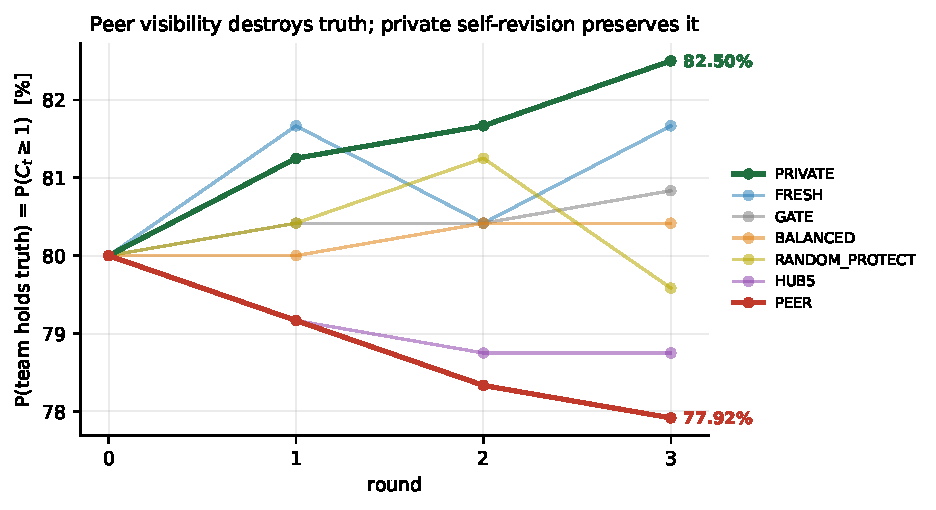
\includegraphics[width=0.82\textwidth]{figs/f1_coverage.pdf}
\caption{P(at least one of five agents holds the correct answer), by round. All seven arms start
at exactly 80.00\% because they share a byte-identical round-0 root bank --- an exact paired
design. \textsc{peer} falls to 77.92\%; \textsc{private} rises to 82.50\%. $n = 240$ items,
240 episodes per arm.}
\end{figure}

\subsection{The mechanism: consolidation, not discovery}

\begin{figure}[H]\centering
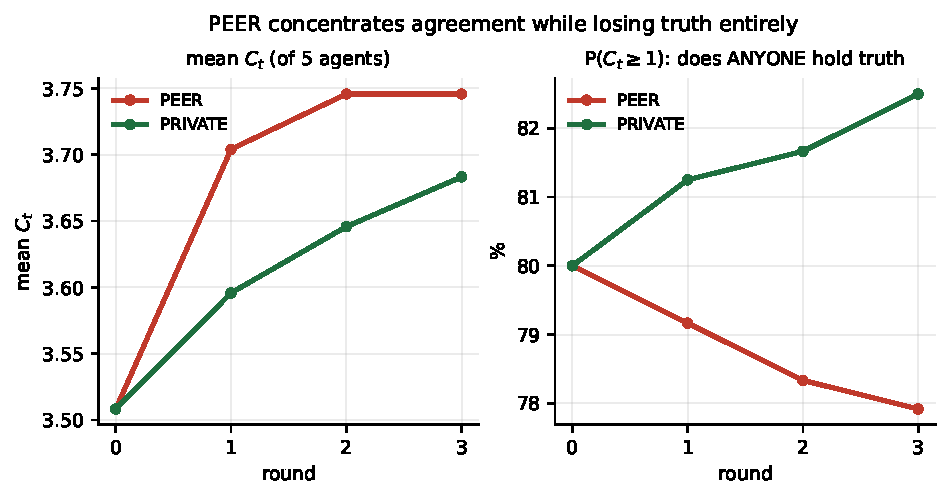
\includegraphics[width=0.94\textwidth]{figs/f2_dissociation.pdf}
\caption{The dissociation that names the mechanism. Under \textsc{peer} the \emph{mean} number of
correct agents \textbf{rises} ($3.508 \rightarrow 3.746$) while the probability that \emph{anyone}
is correct \textbf{falls} ($80.00 \rightarrow 77.92\%$). Communication amplifies whatever the
plurality already holds.}
\end{figure}

\begin{takeaway}{Both absorbing corners at once}
The top-ranked finding of the characterization generalizes this beyond the registered contrast.
Wrong-unanimity prevalence \emph{rises} $+5.40$\,pp\ci{+3.47}{+7.61} in the five packet-passing
arms and is flat in both zero-packet arms (\textsc{private} $-0.74$, \textsc{fresh} $-0.26$, both
null). The root-paired difference-in-differences on covered items gives
\textsc{comm}\,--\,\textsc{private} $= -4.23$\,pp\ci{-6.24}{-2.46} --- independently reproducing
the primary's magnitude from a \emph{different outcome} on a \emph{different panel} (384 items).
\end{takeaway}

\subsection{Consensus is what locks in the error}

\begin{figure}[H]\centering
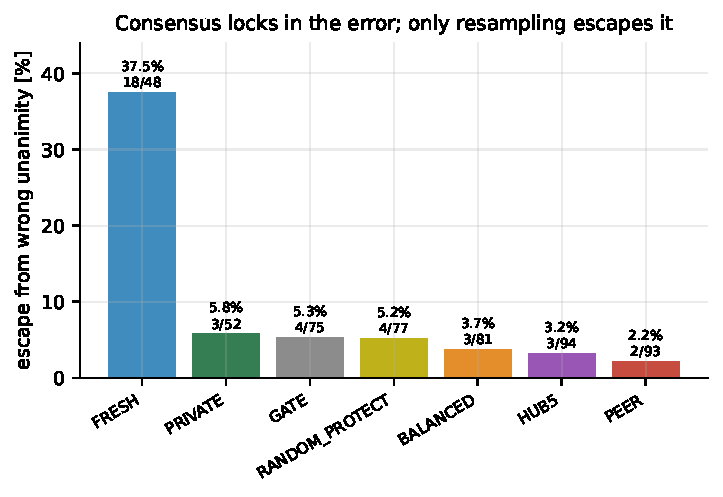
\includegraphics[width=0.78\textwidth]{figs/f5_unanimity.pdf}
\caption{Escape rate from wrong unanimity. Under every communicating protocol a team that agrees on
a wrong answer essentially never recovers (2.2--5.8\%). Under \textsc{fresh} --- independent
resampling with no message passing --- it escapes \textbf{37.5\%} of the time.}
\end{figure}

The comparison localizes the failure precisely. It is not that the model cannot find the answer:
resampling the same model on the same items recovers the truth an order of magnitude more often.
It is that \emph{consensus} is absorbing.

\begin{plainbox}\small
\textbf{A clean structural fact.} Across \textbf{5{,}861 transitions out of any unanimous state} in
the entire study --- correct or wrong, communicating or not --- exactly \textbf{zero} land on a
different unanimous class. Once a team agrees, it never coordinates onto a \emph{new} answer. It
can only decay.
\end{plainbox}

\section{Communication versus sampling}

This is the comparison practitioners actually face: is a team of $k$ agents worth more than $k$
independent samples?

\begin{figure}[H]\centering
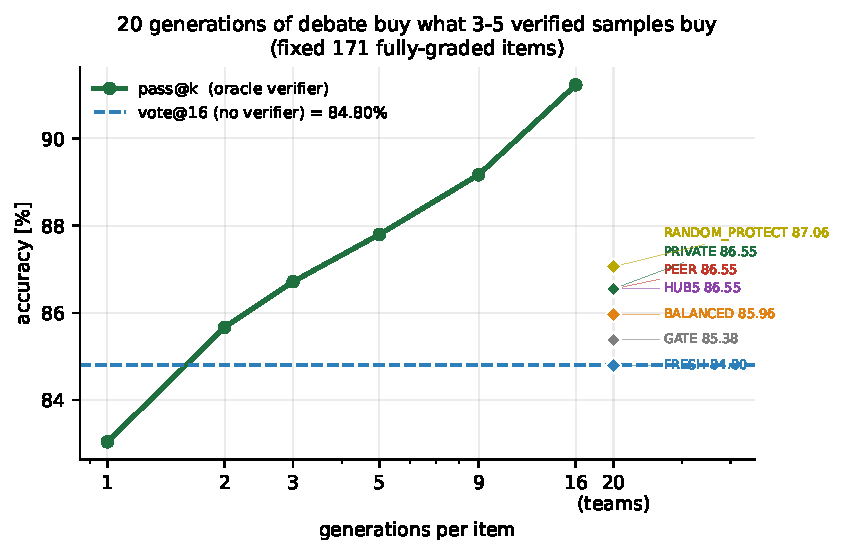
\includegraphics[width=0.86\textwidth]{figs/f4_sampling.pdf}
\caption{Accuracy against generations spent, on the fixed 171-item set where all 16 bank draws are
graded (so both sides use one convention). Every multi-agent arm lands between pass@2 and pass@5
while spending \textbf{20 generations}. \textsc{fresh} at round 3 equals vote@16 \emph{exactly}
(84.80\%).}
\end{figure}

\begin{takeaway}{What debate is worth}
Against an \textbf{oracle verifier}, a 5-agent team running 3 revision rounds (20 generations)
reaches what \textbf{3--5 verified samples} reach --- a 4--7$\times$ compute disadvantage.
Against the achievable comparator \textbf{vote@16} (84.80\%, no verifier), the best arm gains
$\approx 2.3$\,pp. And \textsc{fresh} --- resampling without exchange --- lands exactly on vote@16,
which says the gain comes from \emph{revision}, not from more samples.
\end{takeaway}

\begin{caution}{A measurement trap that nearly produced a false headline}
After the tri-state repair, team accuracy stopped counting ungradeable answers as wrong --- but
\texttt{bank\_summary}'s pass@$k$ still did, because \texttt{bool(None)} is \texttt{False}. The two
halves of this comparison were briefly on \emph{different conventions}, biasing pass@$k$ downward
against the teams. Uncorrected, it would have read as ``revision beats best-of-5.'' A second trap
sits underneath: complete-case pass@$k$ over all 240 items silently shrinks the item set as $k$
grows (236 items at $k{=}1$, only \textbf{171} at $k{=}16$), because a bank needs $k$ graded draws.
Every number above uses the fixed 171-item set.
\end{caution}

\section{What ``revision'' actually consists of}

\begin{figure}[H]\centering
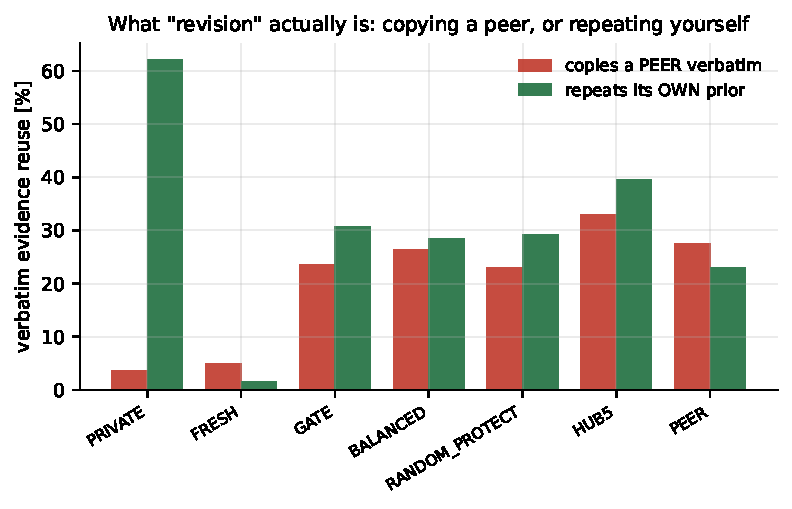
\includegraphics[width=0.86\textwidth]{figs/f6_copying.pdf}
\caption{Verbatim reuse of evidence text between consecutive rounds. Communicating arms import a
peer's evidence byte-identically 23--33\% of the time against a 4.7--4.9\% floor; under
\textsc{private}, agents re-emit \emph{their own} prior evidence \textbf{62\%} of the time.}
\end{figure}

Peer copying is caused by the channel, not by item-level text determinism: a placebo that matches
against a \emph{different episode's} agent on the same item gives 1.1\%, against \textsc{peer}'s
20.4\% in-episode rate. And \textsc{private}'s advantage is not thoughtful reconsideration --- among
agents already holding a correct answer it repeats itself verbatim 70.2\% of the time. The truth is
preserved by \emph{inertia}.

\begin{caution}{A mechanism that failed}
The natural hypothesis --- that correct minorities resist copying and that is why they survive ---
is \textbf{not supported}. Correct minorities do not copy less than the wrong bloc; the point
estimate has the opposite sign and the interval covers zero (peer copy $+0.0367$\ci{-0.0361}{+0.1097},
MDE $0.0677$, 100 paired units). Reported because it was predicted and failed.
\end{caution}

\section{The neural correlate}

\begin{figure}[H]\centering
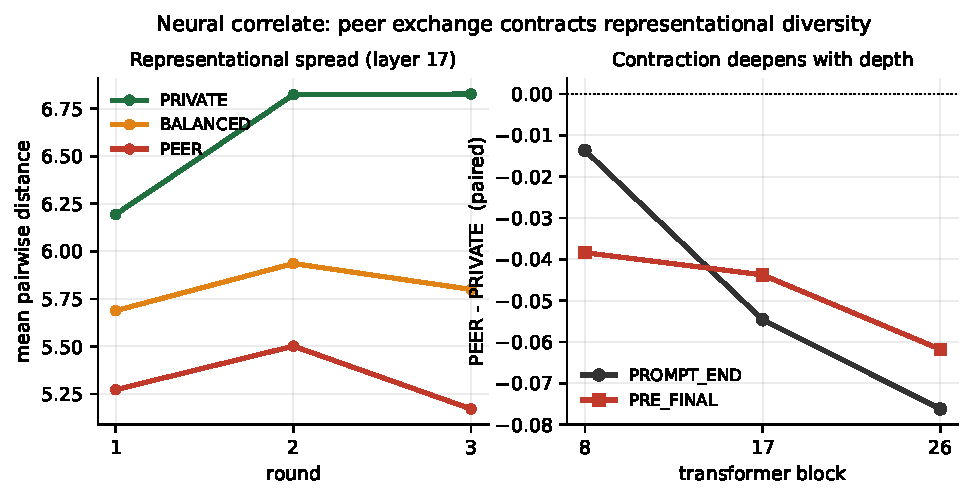
\includegraphics[width=0.94\textwidth]{figs/f7_neural.pdf}
\caption{Residual-stream geometry from teacher-forced replay of 7{,}200 stored decisions (no
regeneration). \textbf{Left:} representational spread across the five agents by round ---
\textsc{peer} contracts, \textsc{private} expands. \textbf{Right:} the paired
\textsc{peer}\,--\,\textsc{private} contraction, by transformer block, at both prospective anchors.}
\end{figure}

Within-item paired \textsc{peer}\,--\,\textsc{private} at round 3, item-clustered bootstrap,
$n = 144$ items (layer 17, \textsc{pre\_final}):

\begin{table}[H]\centering\small
\begin{tabular}{lcc}
\toprule
\textbf{Metric} & \textbf{Effect} & \textbf{95\% CI} \\
\midrule
mean pairwise distance & $-0.0438$ & $[-0.0555, -0.0334]$ \\
max pairwise distance & $-0.0668$ & $[-0.0862, -0.0490]$ \\
leading eigenvalue share & $-0.0548$ & $[-0.0797, -0.0300]$ \\
mean displacement alignment & $+0.0539$ & $[+0.0311, +0.0769]$ \\
\bottomrule
\end{tabular}
\end{table}

The effect holds at \textbf{all six} layer $\times$ anchor combinations, and at \textsc{prompt\_end}
it deepens monotonically with depth ($-0.0136 \rightarrow -0.0546 \rightarrow -0.0762$ across
blocks 8/17/26) --- which rules out a layer-specific artifact. \textsc{balanced}, which hides how
many agents hold each answer, sits between the two ($+0.0169$\ci{+0.0093}{+0.0252} against
\textsc{peer}), in the same direction as its behavioural effect.

\begin{caution}{What this is not}
Descriptive only. No probe, no prediction, no causal claim. A probe separating a correct minority
from its wrong bloc would have \textbf{MDE$_{80}$(AUC) $\approx 0.73$} on this panel --- neither a
hit nor a null would be informative --- so it was not attempted. The geometry and the behaviour are
not independent \emph{evidence}: they describe one process on one set of episodes. Treat it as
mechanism illustration.
\end{caution}

\section{The correct minority}

\begin{takeaway}{Detectable in principle, useless in practice}
Inside a contested, fully-graded team, the correct minority is separated from the wrong bloc by
\texttt{answer\_logprob}: $+0.0220$\ci{+0.0091}{+0.0350} within-team-round paired --- described by
its verifier as ``the most robust thing in the correct-minority panel.'' Self-reported confidence
gives $+0.0115$\ci{+0.0007}{+0.0223}, a fifth of one grid atom. Both are real. Both are far too
small to act on. A flat ``indistinguishable'' null would not survive review, and would be false.

\smallskip
\textbf{Two qualifications the verifier attached, and they matter.} The logprob gap \emph{halves}
to $+0.0115$\ci{+0.0006}{+0.0224} once \texttt{final\_tokens} is controlled --- part of it is
answer length, not conviction. And a placebo that forces the correct bloc to be the \emph{majority}
finds the gap is \emph{larger}, not absent ($n_{\text{correct}}{=}3$:
$+0.0317$\ci{+0.0102}{+0.0533}). So this is a signature of \textbf{correctness in general, not of
minority-ness}. It cannot be used to find embattled correct agents specifically.
\end{takeaway}

Two quantities that are routinely conflated, and must not be:

\begin{itemize}
\item A lone correct agent \textbf{converts at least one teammate in 37.7\%} of rounds (101/268).
\item The team's plurality is correct in only \textbf{22.3\%} of lone-correct rounds (65/291).
\end{itemize}

Persuasion is common. Winning the vote is not.

\section{Where correctness is decided}

The 16-draw bank is generated before any communication, so bank statistics are \emph{exogenous} to
the panel --- the instrument that breaks the circularity of using in-panel accuracy as a difficulty
proxy. Scoring rounds 1--3 only, so bank draws never score themselves:

\begin{plainbox}\small
Minority-correctness concentrates where the bank \emph{contains} the truth but its own plurality
vote \emph{discards} it. At bank \texttt{selection\_gap}${=}1$: $P = 6.10\%$\ci{3.38}{9.02} versus
$0.47\%$\ci{0.21}{0.79} at gap${=}0$ --- a \textbf{13$\times$ rate ratio}, identified without
touching the panel.
\end{plainbox}

\section{The receiver assay}

1{,}280 single-agent probes, previously recorded as \emph{unexecuted}, graded here for the first
time with an independent mod-97 evaluator: \textbf{947 correct / 333 incorrect}.

\begin{table}[H]\centering\small
\caption{Receiver arms. The correct answer is endorsed 4--1 (\textsc{majority}) or 1--4
(\textsc{minority}); \textsc{checked} arms claim verification. $n = 256$ per arm.}
\begin{tabular}{lccc}
\toprule
\textbf{Arm} & \textbf{Accuracy} & \textbf{@1024 tokens} & \textbf{@4096 tokens} \\
\midrule
\textsc{private\_trace} (control) & 0.668 & 0.500 & 0.836 \\
\textsc{minority\_unchecked} & 0.738 & 0.563 & 0.914 \\
\textsc{minority\_checked} & 0.746 & 0.578 & 0.914 \\
\textsc{majority\_checked} & 0.766 & 0.586 & 0.945 \\
\textsc{majority\_unchecked} & 0.781 & 0.586 & 0.977 \\
\bottomrule
\end{tabular}
\end{table}

\begin{takeaway}{Budget dwarfs social framing}
On the control arm alone, quadrupling the thinking budget moves accuracy from \textbf{0.500 to
0.836}. Against that, the entire social manipulation --- whether the correct answer is endorsed by
four peers or one --- is worth $+5.86$\,pp, and a claim of verification is worth nothing
measurable ($-0.39$\,pp\ci{-4.30}{+3.52}). The single largest lever on a reasoning agent in this
study is how long it is allowed to think.
\end{takeaway}

\section{Methodological findings}

\begin{takeaway}{The pairing is doing all the work}
Item ICC is \textbf{0.19--0.84} (design effect $\times$21 to $\times$147). A marginal two-arm
protocol contrast has an MDE of \textbf{0.17--0.29}. The same contrast paired within item has an
MDE of \textbf{0.021--0.029} --- a 6--8$\times$ gain, and the only reason a $-0.046$ effect is
detectable at all. Any multi-agent study that compares arms without pairing on the item is
underpowered by roughly an order of magnitude and will not know it.
\end{takeaway}

\begin{figure}[H]\centering
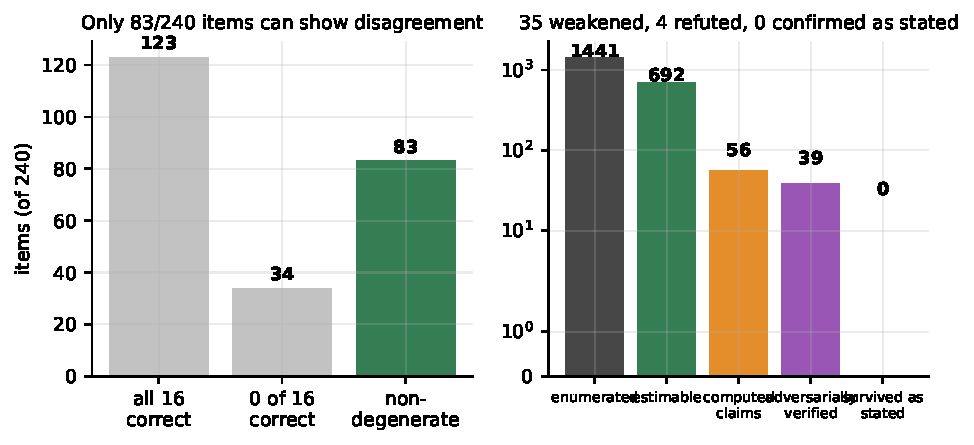
\includegraphics[width=0.94\textwidth]{figs/f8_scope.pdf}
\caption{\textbf{Left:} the panel's usable range --- 123 of 240 items are solved by all 16 draws and
34 by none, leaving \textbf{83} that can express disagreement at all. \textbf{Right:} the
verification funnel, log scale.}
\end{figure}

\paragraph{Composition traps found in this data.} Ungradeable answers coerced to ``wrong'' nearly
\emph{double} the measured truth-loss hazard (13.1\% vs 23.7\% at $C_{t-1}{=}1$). ``Minority
correctness decays over rounds'' is at-risk pool migration, not a trend. A ``switch rate'' read off
\texttt{changed\_class} overstates switching by two thirds. Three of five selectors are structurally
empty, so any ``0 of $N$'' computed on them is an artifact of an absent column.

\paragraph{The panel affords exactly one contrast.} Of 21 protocol pairs, only 12 clear the
minimum-events floor, and 7 of those are null with MDEs of 2.9--5.6\,pp. The significant result is
not selected from many --- there was only ever room for one.

\section{Coverage: what was and was not computed}

\begin{table}[H]\centering\small
\caption{The frozen enumeration manifest. Coverage is arithmetic, not a claim.}
\begin{tabular}{lrr}
\toprule
\textbf{Bucket} & \textbf{Cells} & \textbf{Share} \\
\midrule
Enumerated (131 measurables $\times$ 11 axis roles) & 1{,}441 & 100.0\% \\
\midrule
Estimable & 692 & 48.0\% \\
Structurally void (axis cannot vary in that slice) & 463 & 32.1\% \\
Known-degenerate (censored or determined measures) & 143 & 9.9\% \\
Not estimable (below the events/items floor) & 55 & 3.8\% \\
Redundant & 55 & 3.8\% \\
Identity (algebraically forced) & 33 & 2.3\% \\
\bottomrule
\end{tabular}
\end{table}

Cells pruned as \emph{identity} are worth naming, because each would otherwise look like a finding:
$P(\text{agent correct} \mid n_{\text{correct}}{=}k) = k/5$ exactly; all four minority senses are
subsets of \texttt{correct}${=}1$; protocol differences at round 0 are identically zero, measured
on all 310 shared items.

\section{Limits}

\begin{enumerate}[leftmargin=1.4em]
\item \textbf{One model family, one scale for the main result.} Qwen3-8B carries every headline;
32B ran three protocols on 96 items. Minority-correctness at 32B is \textbf{15 items}, below the
floor --- so nothing minority-conditioned can be said about scale.
\item \textbf{The headline rests on 13 discordant items}, exactly at the minimum for a paired exact
test. It reproduces three ways, but it is one contrast on one family.
\item \textbf{Identification is from randomized protocol assignment, not from the baseline.} Because
round 0 is bit-identical across arms, the pre-registered ``root$\rightarrow$r3 change'' is
algebraically the r3 \emph{level} contrast. The shared root buys variance reduction, not
identification. A reader who takes it for a difference-in-differences has been misled.
\item \textbf{35 of 39 verified claims were weakened.} That is the honest yield of adversarial
verification, and it should temper confidence in the 17 computed claims that were never verified.
\item \textbf{Two things were not run.} The challenge cohort (\textsc{e2c}), which would test the
mechanism interventionally by constructing teams at known initial correct-counts, has only 27
eligible items under the repaired grading rule --- below the testability floor. Spectral entropy
came back null in the geometry tables.
\end{enumerate}

\section{What would falsify this}

The consolidation claim predicts that any manipulation \emph{reducing} a team's exposure to peer
content should preserve coverage, monotonically in dose. Three tests are available and were not run:
\textsc{e2c} at constructed initial correct-counts $C_0 \in \{1,4\}$; the randomized
\texttt{protected} slot extended beyond \textsc{random\_protect}; and a capture of the protected
arm, which would let the geometry contraction be measured under randomized exposure rather than
observationally. If coverage does \emph{not} track exposure dose under those, the mechanism as
stated is wrong.

\vfill
\begin{plainbox}\small
\textbf{Reproduce.} \texttt{PYTHONPATH=src python -m agents\_scaling.ard.compact --run-root \$R
--out-dir tables\_v2}, then \texttt{.minority}, \texttt{.analysis --tables-dir tables\_v2},
\texttt{.keys}, \texttt{.panels --check}. Figures: \texttt{report/figs/}. Full trend table:
\texttt{analysis\_v2/TRENDS.md} (2{,}295 lines). Repair register:
\texttt{docs/ard36/05\_stage0\_repair.md}.
\end{plainbox}

\end{document}
